% Created by tikzDevice version 0.12 on 2019-07-30 11:36:07
% !TEX encoding = UTF-8 Unicode
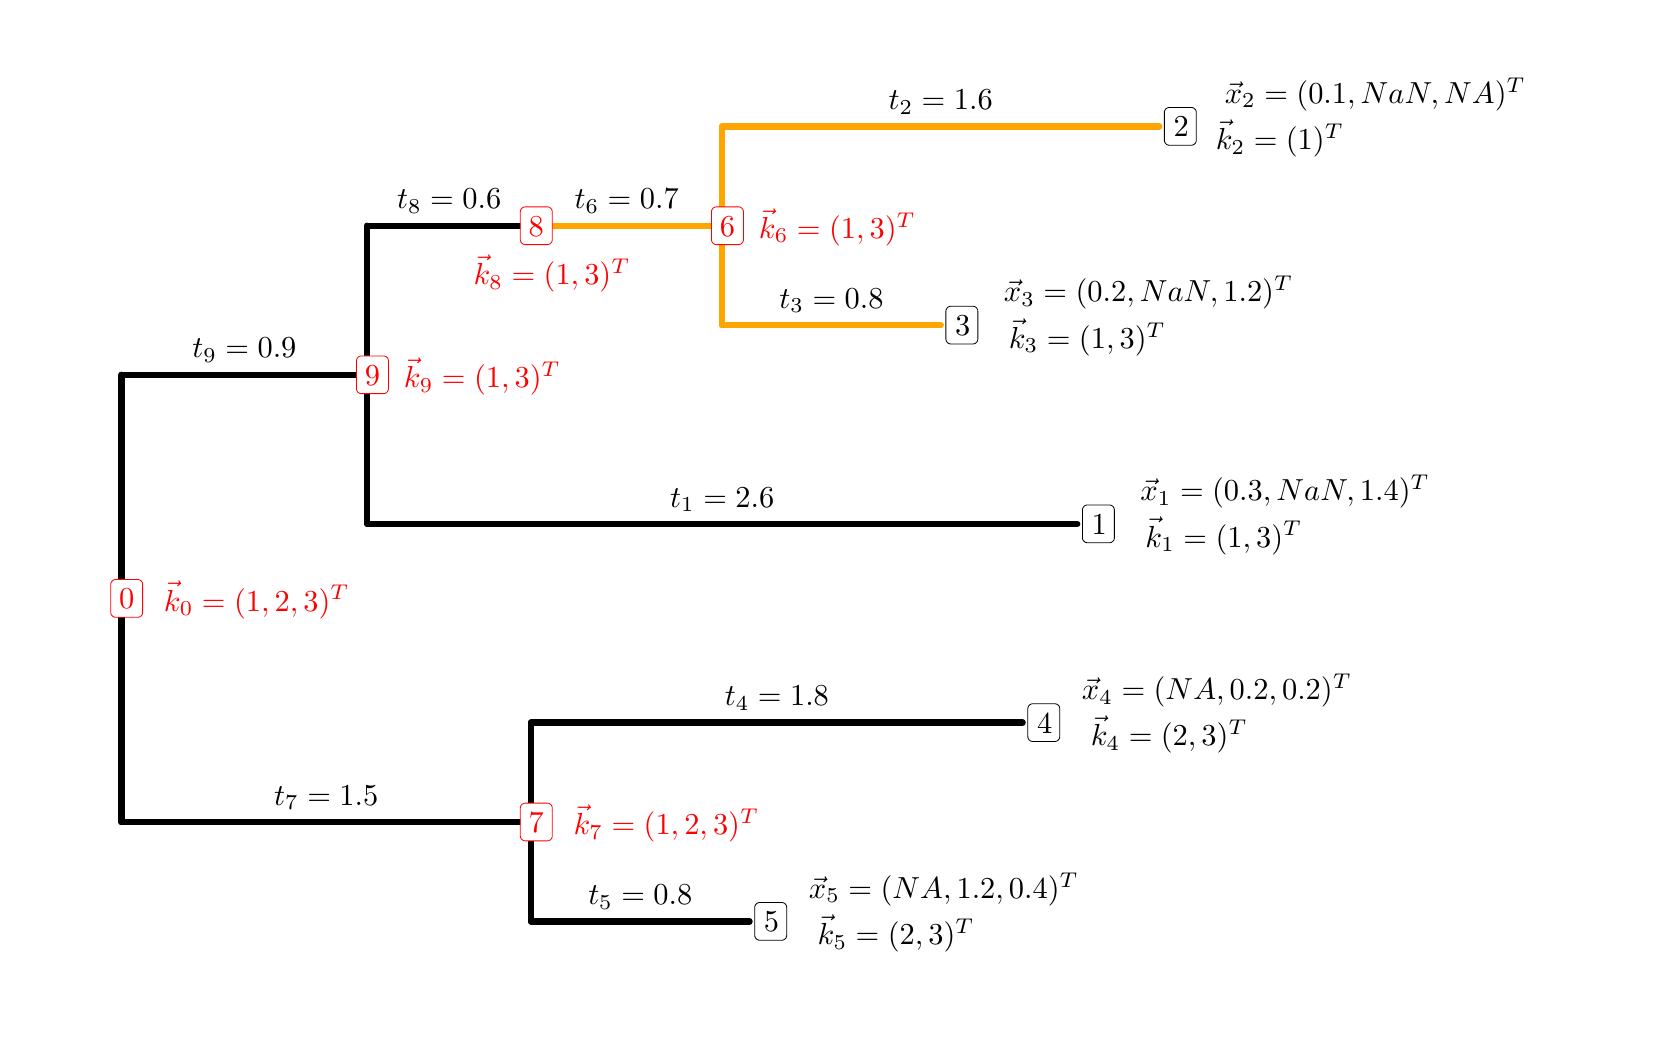
\begin{tikzpicture}[x=1pt,y=1pt]
\definecolor{fillColor}{RGB}{255,255,255}
\path[use as bounding box,fill=fillColor,fill opacity=0.00] (0,0) rectangle (578.16,361.35);
\begin{scope}
\path[clip] (  0.00,  0.00) rectangle (578.16,361.35);
\definecolor{drawColor}{RGB}{255,255,255}
\definecolor{fillColor}{RGB}{255,255,255}

\path[draw=drawColor,line width= 0.6pt,line join=round,line cap=round,fill=fillColor] (  0.00,  0.00) rectangle (578.16,361.35);
\end{scope}
\begin{scope}
\path[clip] (  8.25,  8.25) rectangle (572.66,355.85);
\definecolor{drawColor}{RGB}{255,255,255}
\definecolor{fillColor}{RGB}{255,255,255}

\path[draw=drawColor,line width= 0.6pt,line join=round,line cap=round,fill=fillColor] (  8.25,  8.25) rectangle (572.66,355.85);
\definecolor{drawColor}{RGB}{0,0,0}

\path[draw=drawColor,line width= 2.3pt,line join=round,line cap=round] (181.91, 38.41) -- (260.85, 38.41);

\path[draw=drawColor,line width= 2.3pt,line join=round,line cap=round] (181.91,110.23) -- (359.53,110.23);
\definecolor{drawColor}{RGB}{255,165,0}

\path[draw=drawColor,line width= 2.3pt,line join=round,line cap=round] (250.99,253.87) -- (329.92,253.87);

\path[draw=drawColor,line width= 2.3pt,line join=round,line cap=round] (250.99,325.69) -- (408.86,325.69);
\definecolor{drawColor}{RGB}{0,0,0}

\path[draw=drawColor,line width= 2.3pt,line join=round,line cap=round] (122.71,182.05) -- (379.26,182.05);

\path[draw=drawColor,line width= 2.3pt,line join=round,line cap=round] ( 33.90,155.12) -- ( 33.90,155.12);

\path[draw=drawColor,line width= 2.3pt,line join=round,line cap=round] ( 33.90, 74.32) -- (181.91, 74.32);

\path[draw=drawColor,line width= 2.3pt,line join=round,line cap=round] ( 33.90,235.91) -- (122.71,235.91);

\path[draw=drawColor,line width= 2.3pt,line join=round,line cap=round] (122.71,289.78) -- (181.91,289.78);
\definecolor{drawColor}{RGB}{255,165,0}

\path[draw=drawColor,line width= 2.3pt,line join=round,line cap=round] (181.91,289.78) -- (250.99,289.78);
\definecolor{drawColor}{RGB}{0,0,0}

\path[draw=drawColor,line width= 2.3pt,line join=round,line cap=round] (181.91, 74.32) -- (181.91, 38.41);

\path[draw=drawColor,line width= 2.3pt,line join=round,line cap=round] (181.91, 74.32) -- (181.91,110.23);
\definecolor{drawColor}{RGB}{255,165,0}

\path[draw=drawColor,line width= 2.3pt,line join=round,line cap=round] (250.99,289.78) -- (250.99,253.87);

\path[draw=drawColor,line width= 2.3pt,line join=round,line cap=round] (250.99,289.78) -- (250.99,325.69);
\definecolor{drawColor}{RGB}{0,0,0}

\path[draw=drawColor,line width= 2.3pt,line join=round,line cap=round] (122.71,235.91) -- (122.71,182.05);

\path[draw=drawColor,line width= 2.3pt,line join=round,line cap=round] ( 33.90,155.12) -- ( 33.90,155.12);

\path[draw=drawColor,line width= 2.3pt,line join=round,line cap=round] ( 33.90,155.12) -- ( 33.90, 74.32);

\path[draw=drawColor,line width= 2.3pt,line join=round,line cap=round] ( 33.90,155.12) -- ( 33.90,235.91);

\path[draw=drawColor,line width= 2.3pt,line join=round,line cap=round] (122.71,235.91) -- (122.71,289.78);
\definecolor{drawColor}{RGB}{255,165,0}

\path[draw=drawColor,line width= 2.3pt,line join=round,line cap=round] (181.91,289.78) -- (181.91,289.78);
\definecolor{drawColor}{RGB}{255,0,0}

\path[draw=drawColor,line width= 0.3pt,line join=round,line cap=round,fill=fillColor] ( 31.82,148.31) --
	( 39.74,148.31) --
	( 39.67,148.31) --
	( 39.96,148.32) --
	( 40.25,148.38) --
	( 40.52,148.48) --
	( 40.77,148.63) --
	( 41.00,148.81) --
	( 41.19,149.03) --
	( 41.34,149.27) --
	( 41.46,149.54) --
	( 41.53,149.82) --
	( 41.55,150.11) --
	( 41.55,150.11) --
	( 41.55,160.12) --
	( 41.55,160.12) --
	( 41.53,160.41) --
	( 41.46,160.70) --
	( 41.34,160.96) --
	( 41.19,161.21) --
	( 41.00,161.43) --
	( 40.77,161.61) --
	( 40.52,161.76) --
	( 40.25,161.86) --
	( 39.96,161.92) --
	( 39.74,161.93) --
	( 31.82,161.93) --
	( 32.03,161.92) --
	( 31.74,161.93) --
	( 31.45,161.89) --
	( 31.18,161.81) --
	( 30.91,161.69) --
	( 30.67,161.52) --
	( 30.46,161.32) --
	( 30.29,161.09) --
	( 30.15,160.83) --
	( 30.06,160.56) --
	( 30.02,160.27) --
	( 30.01,160.12) --
	( 30.01,150.11) --
	( 30.02,150.26) --
	( 30.02,149.97) --
	( 30.06,149.68) --
	( 30.15,149.40) --
	( 30.29,149.15) --
	( 30.46,148.91) --
	( 30.67,148.71) --
	( 30.91,148.55) --
	( 31.18,148.42) --
	( 31.45,148.34) --
	( 31.74,148.31) --
	cycle;
\end{scope}
\begin{scope}
\path[clip] (  8.25,  8.25) rectangle (572.66,355.85);
\definecolor{drawColor}{RGB}{255,0,0}

\node[text=drawColor,anchor=base,inner sep=0pt, outer sep=0pt, scale=  1.10] at ( 35.78,151.32) {0};
\definecolor{fillColor}{RGB}{255,255,255}

\path[draw=drawColor,line width= 0.3pt,line join=round,line cap=round,fill=fillColor] (179.83, 67.51) --
	(187.75, 67.51) --
	(187.68, 67.51) --
	(187.97, 67.52) --
	(188.26, 67.58) --
	(188.53, 67.68) --
	(188.78, 67.83) --
	(189.00, 68.01) --
	(189.20, 68.23) --
	(189.35, 68.48) --
	(189.47, 68.74) --
	(189.54, 69.03) --
	(189.56, 69.32) --
	(189.56, 69.32) --
	(189.56, 79.33) --
	(189.56, 79.33) --
	(189.54, 79.62) --
	(189.47, 79.90) --
	(189.35, 80.17) --
	(189.20, 80.41) --
	(189.00, 80.63) --
	(188.78, 80.82) --
	(188.53, 80.96) --
	(188.26, 81.06) --
	(187.97, 81.12) --
	(187.75, 81.14) --
	(179.83, 81.14) --
	(180.04, 81.12) --
	(179.75, 81.13) --
	(179.46, 81.10) --
	(179.18, 81.02) --
	(178.92, 80.89) --
	(178.68, 80.73) --
	(178.47, 80.53) --
	(178.30, 80.29) --
	(178.16, 80.04) --
	(178.07, 79.76) --
	(178.02, 79.47) --
	(178.02, 79.33) --
	(178.02, 69.32) --
	(178.02, 69.46) --
	(178.02, 69.17) --
	(178.07, 68.88) --
	(178.16, 68.61) --
	(178.30, 68.35) --
	(178.47, 68.12) --
	(178.68, 67.92) --
	(178.92, 67.75) --
	(179.18, 67.63) --
	(179.46, 67.55) --
	(179.75, 67.51) --
	cycle;
\end{scope}
\begin{scope}
\path[clip] (  8.25,  8.25) rectangle (572.66,355.85);
\definecolor{drawColor}{RGB}{255,0,0}

\node[text=drawColor,anchor=base,inner sep=0pt, outer sep=0pt, scale=  1.10] at (183.79, 70.52) {7};
\definecolor{fillColor}{RGB}{255,255,255}

\path[draw=drawColor,line width= 0.3pt,line join=round,line cap=round,fill=fillColor] (120.62,229.10) --
	(128.55,229.10) --
	(128.48,229.10) --
	(128.77,229.11) --
	(129.05,229.17) --
	(129.32,229.28) --
	(129.58,229.42) --
	(129.80,229.60) --
	(129.99,229.82) --
	(130.15,230.07) --
	(130.26,230.34) --
	(130.33,230.62) --
	(130.36,230.91) --
	(130.36,230.91) --
	(130.36,240.92) --
	(130.36,240.92) --
	(130.33,241.21) --
	(130.26,241.49) --
	(130.15,241.76) --
	(129.99,242.01) --
	(129.80,242.22) --
	(129.58,242.41) --
	(129.32,242.55) --
	(129.05,242.66) --
	(128.77,242.71) --
	(128.55,242.73) --
	(120.62,242.73) --
	(120.84,242.71) --
	(120.55,242.73) --
	(120.26,242.69) --
	(119.98,242.61) --
	(119.72,242.48) --
	(119.48,242.32) --
	(119.27,242.12) --
	(119.09,241.89) --
	(118.96,241.63) --
	(118.87,241.35) --
	(118.82,241.07) --
	(118.81,240.92) --
	(118.81,230.91) --
	(118.82,231.05) --
	(118.82,230.76) --
	(118.87,230.48) --
	(118.96,230.20) --
	(119.09,229.94) --
	(119.27,229.71) --
	(119.48,229.51) --
	(119.72,229.34) --
	(119.98,229.22) --
	(120.26,229.14) --
	(120.55,229.10) --
	cycle;
\end{scope}
\begin{scope}
\path[clip] (  8.25,  8.25) rectangle (572.66,355.85);
\definecolor{drawColor}{RGB}{255,0,0}

\node[text=drawColor,anchor=base,inner sep=0pt, outer sep=0pt, scale=  1.10] at (124.59,232.11) {9};
\definecolor{fillColor}{RGB}{255,255,255}

\path[draw=drawColor,line width= 0.3pt,line join=round,line cap=round,fill=fillColor] (179.83,282.96) --
	(187.75,282.96) --
	(187.68,282.97) --
	(187.97,282.98) --
	(188.26,283.04) --
	(188.53,283.14) --
	(188.78,283.28) --
	(189.00,283.47) --
	(189.20,283.69) --
	(189.35,283.93) --
	(189.47,284.20) --
	(189.54,284.48) --
	(189.56,284.77) --
	(189.56,284.77) --
	(189.56,294.78) --
	(189.56,294.78) --
	(189.54,295.07) --
	(189.47,295.36) --
	(189.35,295.62) --
	(189.20,295.87) --
	(189.00,296.09) --
	(188.78,296.27) --
	(188.53,296.42) --
	(188.26,296.52) --
	(187.97,296.58) --
	(187.75,296.59) --
	(179.83,296.59) --
	(180.04,296.58) --
	(179.75,296.59) --
	(179.46,296.55) --
	(179.18,296.47) --
	(178.92,296.35) --
	(178.68,296.18) --
	(178.47,295.98) --
	(178.30,295.75) --
	(178.16,295.49) --
	(178.07,295.22) --
	(178.02,294.93) --
	(178.02,294.78) --
	(178.02,284.77) --
	(178.02,284.92) --
	(178.02,284.63) --
	(178.07,284.34) --
	(178.16,284.06) --
	(178.30,283.81) --
	(178.47,283.57) --
	(178.68,283.37) --
	(178.92,283.21) --
	(179.18,283.08) --
	(179.46,283.00) --
	(179.75,282.97) --
	cycle;
\end{scope}
\begin{scope}
\path[clip] (  8.25,  8.25) rectangle (572.66,355.85);
\definecolor{drawColor}{RGB}{255,0,0}

\node[text=drawColor,anchor=base,inner sep=0pt, outer sep=0pt, scale=  1.10] at (183.79,285.98) {8};
\definecolor{fillColor}{RGB}{255,255,255}

\path[draw=drawColor,line width= 0.3pt,line join=round,line cap=round,fill=fillColor] (248.90,282.96) --
	(256.82,282.96) --
	(256.75,282.97) --
	(257.04,282.98) --
	(257.33,283.04) --
	(257.60,283.14) --
	(257.85,283.28) --
	(258.08,283.47) --
	(258.27,283.69) --
	(258.42,283.93) --
	(258.54,284.20) --
	(258.61,284.48) --
	(258.63,284.77) --
	(258.63,284.77) --
	(258.63,294.78) --
	(258.63,294.78) --
	(258.61,295.07) --
	(258.54,295.36) --
	(258.42,295.62) --
	(258.27,295.87) --
	(258.08,296.09) --
	(257.85,296.27) --
	(257.60,296.42) --
	(257.33,296.52) --
	(257.04,296.58) --
	(256.82,296.59) --
	(248.90,296.59) --
	(249.11,296.58) --
	(248.82,296.59) --
	(248.54,296.55) --
	(248.26,296.47) --
	(247.99,296.35) --
	(247.75,296.18) --
	(247.54,295.98) --
	(247.37,295.75) --
	(247.23,295.49) --
	(247.14,295.22) --
	(247.10,294.93) --
	(247.09,294.78) --
	(247.09,284.77) --
	(247.10,284.92) --
	(247.10,284.63) --
	(247.14,284.34) --
	(247.23,284.06) --
	(247.37,283.81) --
	(247.54,283.57) --
	(247.75,283.37) --
	(247.99,283.21) --
	(248.26,283.08) --
	(248.54,283.00) --
	(248.82,282.97) --
	cycle;
\end{scope}
\begin{scope}
\path[clip] (  8.25,  8.25) rectangle (572.66,355.85);
\definecolor{drawColor}{RGB}{255,0,0}

\node[text=drawColor,anchor=base,inner sep=0pt, outer sep=0pt, scale=  1.10] at (252.86,285.98) {6};
\definecolor{drawColor}{RGB}{0,0,0}
\definecolor{fillColor}{RGB}{255,255,255}

\path[draw=drawColor,line width= 0.3pt,line join=round,line cap=round,fill=fillColor] (264.53, 31.60) --
	(272.46, 31.60) --
	(272.39, 31.60) --
	(272.68, 31.61) --
	(272.96, 31.67) --
	(273.24, 31.78) --
	(273.49, 31.92) --
	(273.71, 32.10) --
	(273.91, 32.32) --
	(274.06, 32.57) --
	(274.18, 32.84) --
	(274.25, 33.12) --
	(274.27, 33.41) --
	(274.27, 33.41) --
	(274.27, 43.42) --
	(274.27, 43.42) --
	(274.25, 43.71) --
	(274.18, 43.99) --
	(274.06, 44.26) --
	(273.91, 44.51) --
	(273.71, 44.72) --
	(273.49, 44.91) --
	(273.24, 45.05) --
	(272.96, 45.16) --
	(272.68, 45.21) --
	(272.46, 45.23) --
	(264.53, 45.23) --
	(264.75, 45.21) --
	(264.46, 45.23) --
	(264.17, 45.19) --
	(263.89, 45.11) --
	(263.63, 44.98) --
	(263.39, 44.82) --
	(263.18, 44.62) --
	(263.01, 44.39) --
	(262.87, 44.13) --
	(262.78, 43.85) --
	(262.73, 43.57) --
	(262.73, 43.42) --
	(262.73, 33.41) --
	(262.73, 33.55) --
	(262.73, 33.26) --
	(262.78, 32.98) --
	(262.87, 32.70) --
	(263.01, 32.44) --
	(263.18, 32.21) --
	(263.39, 32.01) --
	(263.63, 31.84) --
	(263.89, 31.72) --
	(264.17, 31.64) --
	(264.46, 31.60) --
	cycle;
\end{scope}
\begin{scope}
\path[clip] (  8.25,  8.25) rectangle (572.66,355.85);
\definecolor{drawColor}{RGB}{0,0,0}

\node[text=drawColor,anchor=base west,inner sep=0pt, outer sep=0pt, scale=  1.10] at (266.05, 34.61) {5};
\definecolor{fillColor}{RGB}{255,255,255}

\path[draw=drawColor,line width= 0.3pt,line join=round,line cap=round,fill=fillColor] (363.21,103.42) --
	(371.14,103.42) --
	(371.06,103.42) --
	(371.35,103.43) --
	(371.64,103.49) --
	(371.91,103.59) --
	(372.16,103.74) --
	(372.39,103.92) --
	(372.58,104.14) --
	(372.74,104.39) --
	(372.85,104.65) --
	(372.92,104.94) --
	(372.94,105.23) --
	(372.94,105.23) --
	(372.94,115.24) --
	(372.94,115.24) --
	(372.92,115.53) --
	(372.85,115.81) --
	(372.74,116.08) --
	(372.58,116.32) --
	(372.39,116.54) --
	(372.16,116.72) --
	(371.91,116.87) --
	(371.64,116.97) --
	(371.35,117.03) --
	(371.14,117.04) --
	(363.21,117.04) --
	(363.43,117.03) --
	(363.13,117.04) --
	(362.85,117.01) --
	(362.57,116.93) --
	(362.30,116.80) --
	(362.07,116.64) --
	(361.86,116.44) --
	(361.68,116.20) --
	(361.55,115.95) --
	(361.45,115.67) --
	(361.41,115.38) --
	(361.40,115.24) --
	(361.40,105.23) --
	(361.41,105.37) --
	(361.41,105.08) --
	(361.45,104.79) --
	(361.55,104.52) --
	(361.68,104.26) --
	(361.86,104.03) --
	(362.07,103.83) --
	(362.30,103.66) --
	(362.57,103.54) --
	(362.85,103.46) --
	(363.13,103.42) --
	cycle;
\end{scope}
\begin{scope}
\path[clip] (  8.25,  8.25) rectangle (572.66,355.85);
\definecolor{drawColor}{RGB}{0,0,0}

\node[text=drawColor,anchor=base west,inner sep=0pt, outer sep=0pt, scale=  1.10] at (364.73,106.43) {4};
\definecolor{fillColor}{RGB}{255,255,255}

\path[draw=drawColor,line width= 0.3pt,line join=round,line cap=round,fill=fillColor] (333.61,247.06) --
	(341.53,247.06) --
	(341.46,247.06) --
	(341.75,247.07) --
	(342.04,247.13) --
	(342.31,247.23) --
	(342.56,247.38) --
	(342.79,247.56) --
	(342.98,247.78) --
	(343.13,248.02) --
	(343.25,248.29) --
	(343.32,248.57) --
	(343.34,248.86) --
	(343.34,248.86) --
	(343.34,258.87) --
	(343.34,258.87) --
	(343.32,259.16) --
	(343.25,259.45) --
	(343.13,259.71) --
	(342.98,259.96) --
	(342.79,260.18) --
	(342.56,260.36) --
	(342.31,260.51) --
	(342.04,260.61) --
	(341.75,260.67) --
	(341.53,260.68) --
	(333.61,260.68) --
	(333.82,260.67) --
	(333.53,260.68) --
	(333.24,260.64) --
	(332.97,260.56) --
	(332.70,260.44) --
	(332.46,260.27) --
	(332.25,260.07) --
	(332.08,259.84) --
	(331.94,259.58) --
	(331.85,259.31) --
	(331.80,259.02) --
	(331.80,258.87) --
	(331.80,248.86) --
	(331.80,249.01) --
	(331.80,248.72) --
	(331.85,248.43) --
	(331.94,248.15) --
	(332.08,247.90) --
	(332.25,247.66) --
	(332.46,247.46) --
	(332.70,247.30) --
	(332.97,247.17) --
	(333.24,247.09) --
	(333.53,247.06) --
	cycle;
\end{scope}
\begin{scope}
\path[clip] (  8.25,  8.25) rectangle (572.66,355.85);
\definecolor{drawColor}{RGB}{0,0,0}

\node[text=drawColor,anchor=base west,inner sep=0pt, outer sep=0pt, scale=  1.10] at (335.12,250.07) {3};
\definecolor{fillColor}{RGB}{255,255,255}

\path[draw=drawColor,line width= 0.3pt,line join=round,line cap=round,fill=fillColor] (412.54,318.87) --
	(420.47,318.87) --
	(420.40,318.87) --
	(420.69,318.89) --
	(420.97,318.94) --
	(421.25,319.05) --
	(421.50,319.19) --
	(421.72,319.38) --
	(421.92,319.59) --
	(422.07,319.84) --
	(422.19,320.11) --
	(422.26,320.39) --
	(422.28,320.68) --
	(422.28,320.68) --
	(422.28,330.69) --
	(422.28,330.69) --
	(422.26,330.98) --
	(422.19,331.26) --
	(422.07,331.53) --
	(421.92,331.78) --
	(421.72,332.00) --
	(421.50,332.18) --
	(421.25,332.32) --
	(420.97,332.43) --
	(420.69,332.49) --
	(420.47,332.50) --
	(412.54,332.50) --
	(412.76,332.49) --
	(412.47,332.50) --
	(412.18,332.46) --
	(411.90,332.38) --
	(411.64,332.26) --
	(411.40,332.09) --
	(411.19,331.89) --
	(411.02,331.66) --
	(410.88,331.40) --
	(410.79,331.12) --
	(410.74,330.84) --
	(410.74,330.69) --
	(410.74,320.68) --
	(410.74,320.83) --
	(410.74,320.53) --
	(410.79,320.25) --
	(410.88,319.97) --
	(411.02,319.71) --
	(411.19,319.48) --
	(411.40,319.28) --
	(411.64,319.12) --
	(411.90,318.99) --
	(412.18,318.91) --
	(412.47,318.87) --
	cycle;
\end{scope}
\begin{scope}
\path[clip] (  8.25,  8.25) rectangle (572.66,355.85);
\definecolor{drawColor}{RGB}{0,0,0}

\node[text=drawColor,anchor=base west,inner sep=0pt, outer sep=0pt, scale=  1.10] at (414.06,321.88) {2};
\definecolor{fillColor}{RGB}{255,255,255}

\path[draw=drawColor,line width= 0.3pt,line join=round,line cap=round,fill=fillColor] (382.94,175.24) --
	(390.87,175.24) --
	(390.80,175.24) --
	(391.09,175.25) --
	(391.37,175.31) --
	(391.64,175.41) --
	(391.90,175.56) --
	(392.12,175.74) --
	(392.31,175.96) --
	(392.47,176.20) --
	(392.58,176.47) --
	(392.65,176.75) --
	(392.68,177.04) --
	(392.68,177.04) --
	(392.68,187.06) --
	(392.68,187.06) --
	(392.65,187.35) --
	(392.58,187.63) --
	(392.47,187.90) --
	(392.31,188.14) --
	(392.12,188.36) --
	(391.90,188.54) --
	(391.64,188.69) --
	(391.37,188.79) --
	(391.09,188.85) --
	(390.87,188.86) --
	(382.94,188.86) --
	(383.16,188.85) --
	(382.87,188.86) --
	(382.58,188.83) --
	(382.30,188.75) --
	(382.04,188.62) --
	(381.80,188.46) --
	(381.59,188.25) --
	(381.42,188.02) --
	(381.28,187.76) --
	(381.19,187.49) --
	(381.14,187.20) --
	(381.14,187.06) --
	(381.14,177.04) --
	(381.14,177.19) --
	(381.14,176.90) --
	(381.19,176.61) --
	(381.28,176.34) --
	(381.42,176.08) --
	(381.59,175.85) --
	(381.80,175.64) --
	(382.04,175.48) --
	(382.30,175.35) --
	(382.58,175.27) --
	(382.87,175.24) --
	cycle;
\end{scope}
\begin{scope}
\path[clip] (  8.25,  8.25) rectangle (572.66,355.85);
\definecolor{drawColor}{RGB}{0,0,0}

\node[text=drawColor,anchor=base west,inner sep=0pt, outer sep=0pt, scale=  1.10] at (384.46,178.25) {1};

\node[text=drawColor,anchor=base west,inner sep=0pt, outer sep=0pt, scale=  1.10] at (282.31, 46.78) {$\vec{x}_{5}=(NA, 1.2, 0.4)^T$};

\node[text=drawColor,anchor=base west,inner sep=0pt, outer sep=0pt, scale=  1.10] at (380.98,118.60) {$\vec{x}_{4}=(NA, 0.2, 0.2)^T$};

\node[text=drawColor,anchor=base west,inner sep=0pt, outer sep=0pt, scale=  1.10] at (352.78,262.23) {$\vec{x}_{3}=(0.2, NaN, 1.2)^T$};

\node[text=drawColor,anchor=base west,inner sep=0pt, outer sep=0pt, scale=  1.10] at (432.57,334.05) {$\vec{x}_{2}=(0.1, NaN, NA)^T$};

\node[text=drawColor,anchor=base west,inner sep=0pt, outer sep=0pt, scale=  1.10] at (402.12,190.41) {$\vec{x}_{1}=(0.3, NaN, 1.4)^T$};

\node[text=drawColor,anchor=base west,inner sep=0pt, outer sep=0pt, scale=  1.10] at (285.49, 30.05) {$\vec{k}_{5}=(2, 3)^T$};

\node[text=drawColor,anchor=base west,inner sep=0pt, outer sep=0pt, scale=  1.10] at (384.16,101.87) {$\vec{k}_{4}=(2, 3)^T$};

\node[text=drawColor,anchor=base west,inner sep=0pt, outer sep=0pt, scale=  1.10] at (354.56,245.50) {$\vec{k}_{3}=(1, 3)^T$};

\node[text=drawColor,anchor=base west,inner sep=0pt, outer sep=0pt, scale=  1.10] at (429.33,317.32) {$\vec{k}_{2}=(1)^T$};

\node[text=drawColor,anchor=base west,inner sep=0pt, outer sep=0pt, scale=  1.10] at (403.90,173.69) {$\vec{k}_{1}=(1, 3)^T$};
\definecolor{drawColor}{RGB}{255,0,0}

\node[text=drawColor,anchor=base west,inner sep=0pt, outer sep=0pt, scale=  1.10] at ( 49.25,150.56) {$\vec{k}_{0}=(1, 2, 3)^T$};

\node[text=drawColor,anchor=base west,inner sep=0pt, outer sep=0pt, scale=  1.10] at (197.26, 69.76) {$\vec{k}_{7}=(1, 2, 3)^T$};

\node[text=drawColor,anchor=base west,inner sep=0pt, outer sep=0pt, scale=  1.10] at (135.97,231.35) {$\vec{k}_{9}=(1, 3)^T$};

\node[text=drawColor,anchor=base west,inner sep=0pt, outer sep=0pt, scale=  1.10] at (264.24,285.22) {$\vec{k}_{6}=(1, 3)^T$};

\node[text=drawColor,anchor=base,inner sep=0pt, outer sep=0pt, scale=  1.10] at (189.48,268.49) {$\vec{k}_{8}=(1, 3)^T$};
\definecolor{drawColor}{RGB}{0,0,0}

\node[text=drawColor,anchor=base,inner sep=0pt, outer sep=0pt, scale=  1.10] at (221.38, 44.50) {$t_{5}=0.8$};

\node[text=drawColor,anchor=base,inner sep=0pt, outer sep=0pt, scale=  1.10] at (270.72,116.31) {$t_{4}=1.8$};

\node[text=drawColor,anchor=base,inner sep=0pt, outer sep=0pt, scale=  1.10] at (290.46,259.95) {$t_{3}=0.8$};

\node[text=drawColor,anchor=base,inner sep=0pt, outer sep=0pt, scale=  1.10] at (329.92,331.77) {$t_{2}=1.6$};

\node[text=drawColor,anchor=base,inner sep=0pt, outer sep=0pt, scale=  1.10] at (250.99,188.13) {$t_{1}=2.6$};

\node[text=drawColor,anchor=base,inner sep=0pt, outer sep=0pt, scale=  1.10] at (107.91, 80.41) {$t_{7}=1.5$};

\node[text=drawColor,anchor=base,inner sep=0pt, outer sep=0pt, scale=  1.10] at ( 78.31,242.00) {$t_{9}=0.9$};

\node[text=drawColor,anchor=base,inner sep=0pt, outer sep=0pt, scale=  1.10] at (152.31,295.86) {$t_{8}=0.6$};

\node[text=drawColor,anchor=base,inner sep=0pt, outer sep=0pt, scale=  1.10] at (216.45,295.86) {$t_{6}=0.7$};
\end{scope}
\end{tikzpicture}
